%!TEX root = ../thesis.tex

\chapter{Multi-detector wavelength calibration} % Main appendix title
\label{appendix:wavelength_fitting}

In this Appendix we provide an example of multi-detector wavelength calibration.
This is to try and improve the wavelength calibration on the detectors in which a limited number of telluric lines fall.

The spectrum recorded across the four detectors is created from a single dispersion and should, in theory, be able to be modelled by a single polynomial. \cref{fig:multidectorfit} shows the pixel-wavelength calibrating points for the 4 detectors, along with the individual fits, extended over the four detectors. At this scale all four lines are basically similar except for the fourth detector near  the wavelength region of detector 1 where it is slightly higher. On top is also a line indicating a polynomial fit made using the points from all four detectors and including the fixed gaps between detectors. 

\cref{fig:multidectorfitdiff} shows the difference between the individual detectors and the combined fit. Within the individual detectors the absolute wavelength difference is less than 0.5\nm{} at the edges of detector one, however the differences exceed 0.3\nm outside of the original detector. They are quadratic in shape as they are the difference between two quadratics.

\begin{figure}
    \centering
    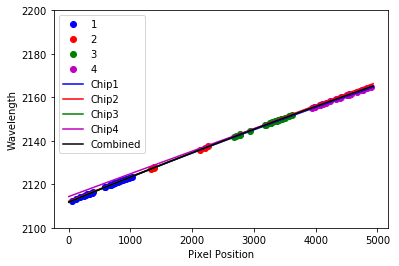
\includegraphics[width=0.75\linewidth]{./figures/appendix/multi_detector_fit}
    \caption[Multi-detector fit and difference to individual fits.]{ Fit of each individual detector along with a combined quadratic fit with fixed detector gaps.}
    \label{fig:multidectorfit}
\end{figure}


\begin{figure}
    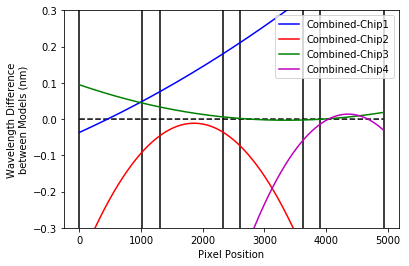
\includegraphics[width=0.75\linewidth]{./figures/appendix/multidector_fit_diff}
    \caption[Multi-detector difference of combined fit to the individual fits.]{Multi-detector difference of each individual fit from the combined detector fit.}
    \label{fig:multidectorfitdiff}
\end{figure}

The combined fit is made by first assigning each horizontal pixel of each detector the position between 0 and 4095 in pixel coordinates of the {CRIRES} detectors.
A transformation is made into a psudo-physical pixel coordinates from the left edge of the first detector by including the gaps between the detectors (in pixels).
The parameters \(gap_{1}\), \(gap_{2}\), \(gap_{3}\) are the 3 gaps between neighbouring detectors gaps and are defined in pixel space as follows:
\[
gap =\begin{cases}
0,                       & ~~~~0=<pxl<1024\\
gap_1,                    & 1024=<pxl<2048\\
gap_1 + gap_2,             & 2048=<pxl<3072\\
gap_1 + gap_2 + gap_3,      & 3072=<pxl<4096
\end{cases}
\]

The pixel widths of these gaps can be fixed to known values (e.g.\ 282, 278, and 275 pixels~\citep{brogi_rotation_2016}) or allowed to vary and included in the fitting process.


\subsection{Comparing the variable gaps}

\missingfigure{Corner plot fixed gaps}

\missingfigure{Corner plot variable gaps}


\begin{figure}
    \centering
    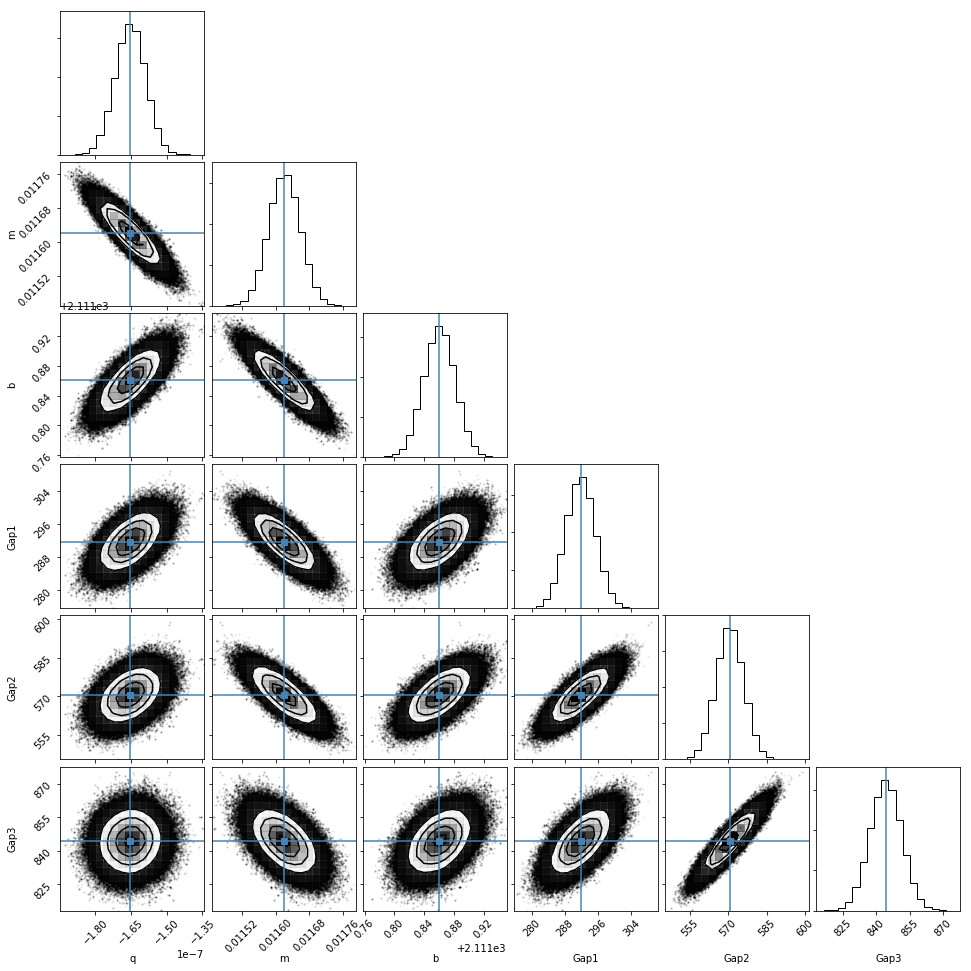
\includegraphics[width=0.5\linewidth]{./figures/appendix/multidetecot_param_fit}
    \caption[Multi-detector parameter correlations.]{Corner plot of emcee combined fitting.
    The elliptical point clouds indicate there are correlations between parameters.}
    \label{fig:multidetecotparamfit}
\end{figure}

This example does not include the height on the detectors the spectrum falls or any skewness of the spectrum to pixel rows or any miss-alignment between the detectors. All which could have some affect on a global wavelength calibration.

\cref{tab:example_calibration_parametres} shows the parameters obtained as well as a fit statistic for quadratic and cubic fitting. \textbf{BIC shows that}

\todo{remove vertical lines}
\todo{fill in table}
\begin{table}
    \small
    \caption[Example of multi-detector fitting parameters.]{Example of multi-detector fitting parameters obtained for HD\,30501 observation 2 under different scenarios.}
    \begin{tabular}{|l|c|c|c|c|c|c|c|c|c|c|c|c|}
    	\toprule
    	  &    \multicolumn{8}{c|}{Individual Detectors}    &    \multicolumn{4}{c|}{Combined}    \\
    	  & \multicolumn{2}{c|}{\#1} & \multicolumn{2}{c|}{\#2} & \multicolumn{2}{c|}{\#3} & \multicolumn{2}{c|}{\#4} & \multicolumn{2}{c|}{Fixed Gaps} & \multicolumn{2}{c|}{Variable Gaps} \\ \midrule
    	a3 (u)    &  -   &    1e-4    &  -   &    &  -   &    &  -   &    &  -   &    &  -   &    blah    \\
    	a2 (q)    &      &    &    &    &    &    &    &    &    &    &    &    blah    \\
    	a1 (m)   &      &    &    &    &    &    &    &    &    &    &    &    blah    \\
    	a0 (b)    & 2111 &    2111    & 2111 &    2111    & 2111 &    2111    & 2111 &    2111    & 2111 &    2111    & 2111 & blah \\
        \(gap_{1}\) &      &    &    &    &    &    &    &    &   1367  & 1367   &   & x\\
        \(gap_{2}\) &      &    &    &    &    &    &    &    &  2700   &  2700  &   & x\\
        \(gap_{3}\) &      &    &    &    &    &    &    &    &   3900 &   3900 &    & x\\
    	\textchisquared{} &    &    &    &    &    &    &    &    &    &    &    &    blah    \\
    	BIC        & -234      &    -234    & -234 &    -234    & -234 &    -234    &    &    -234    & -234 &    -234    & -234 &    blah  \\
        \bottomrule
    \end{tabular}\label{tab:example_calibration_parametres}
\end{table}


\missingfigure{Residuals between individual fitting and the variable gap fits}
